Рассмотрим описанные алгоритмы поиска маршрута. Пусть поиск производится по квадратной матрице растояний $D$ размером $N$.

\section{Поиск полным перебором}
Алгоритм начинает в 0-й вершине и передаёт в рекурсивную функцию текущую позицию и список доступных вершин, содержащий все вершины кроме начальной. Далее функция поочерёдно производит выбор каждой из возможных вершин в качестве следующей для перехода, учитывает расстояние от предыдущей вершины и вызывает эту же функцию, исключив из списка доступных вершин выбранную. Функция возвращает наиболее короткий путь из всех найденых вариантов, после чего добавляет в него текущую вершину и возвращает в качестве самого короткого пути. Функция, получившая пустое множество доступных вершин совершает переход в начальную вершину.

Схема алгоритма приведена на рисунке 2.1
\begin{figure}[h]
	\begin{center}
		{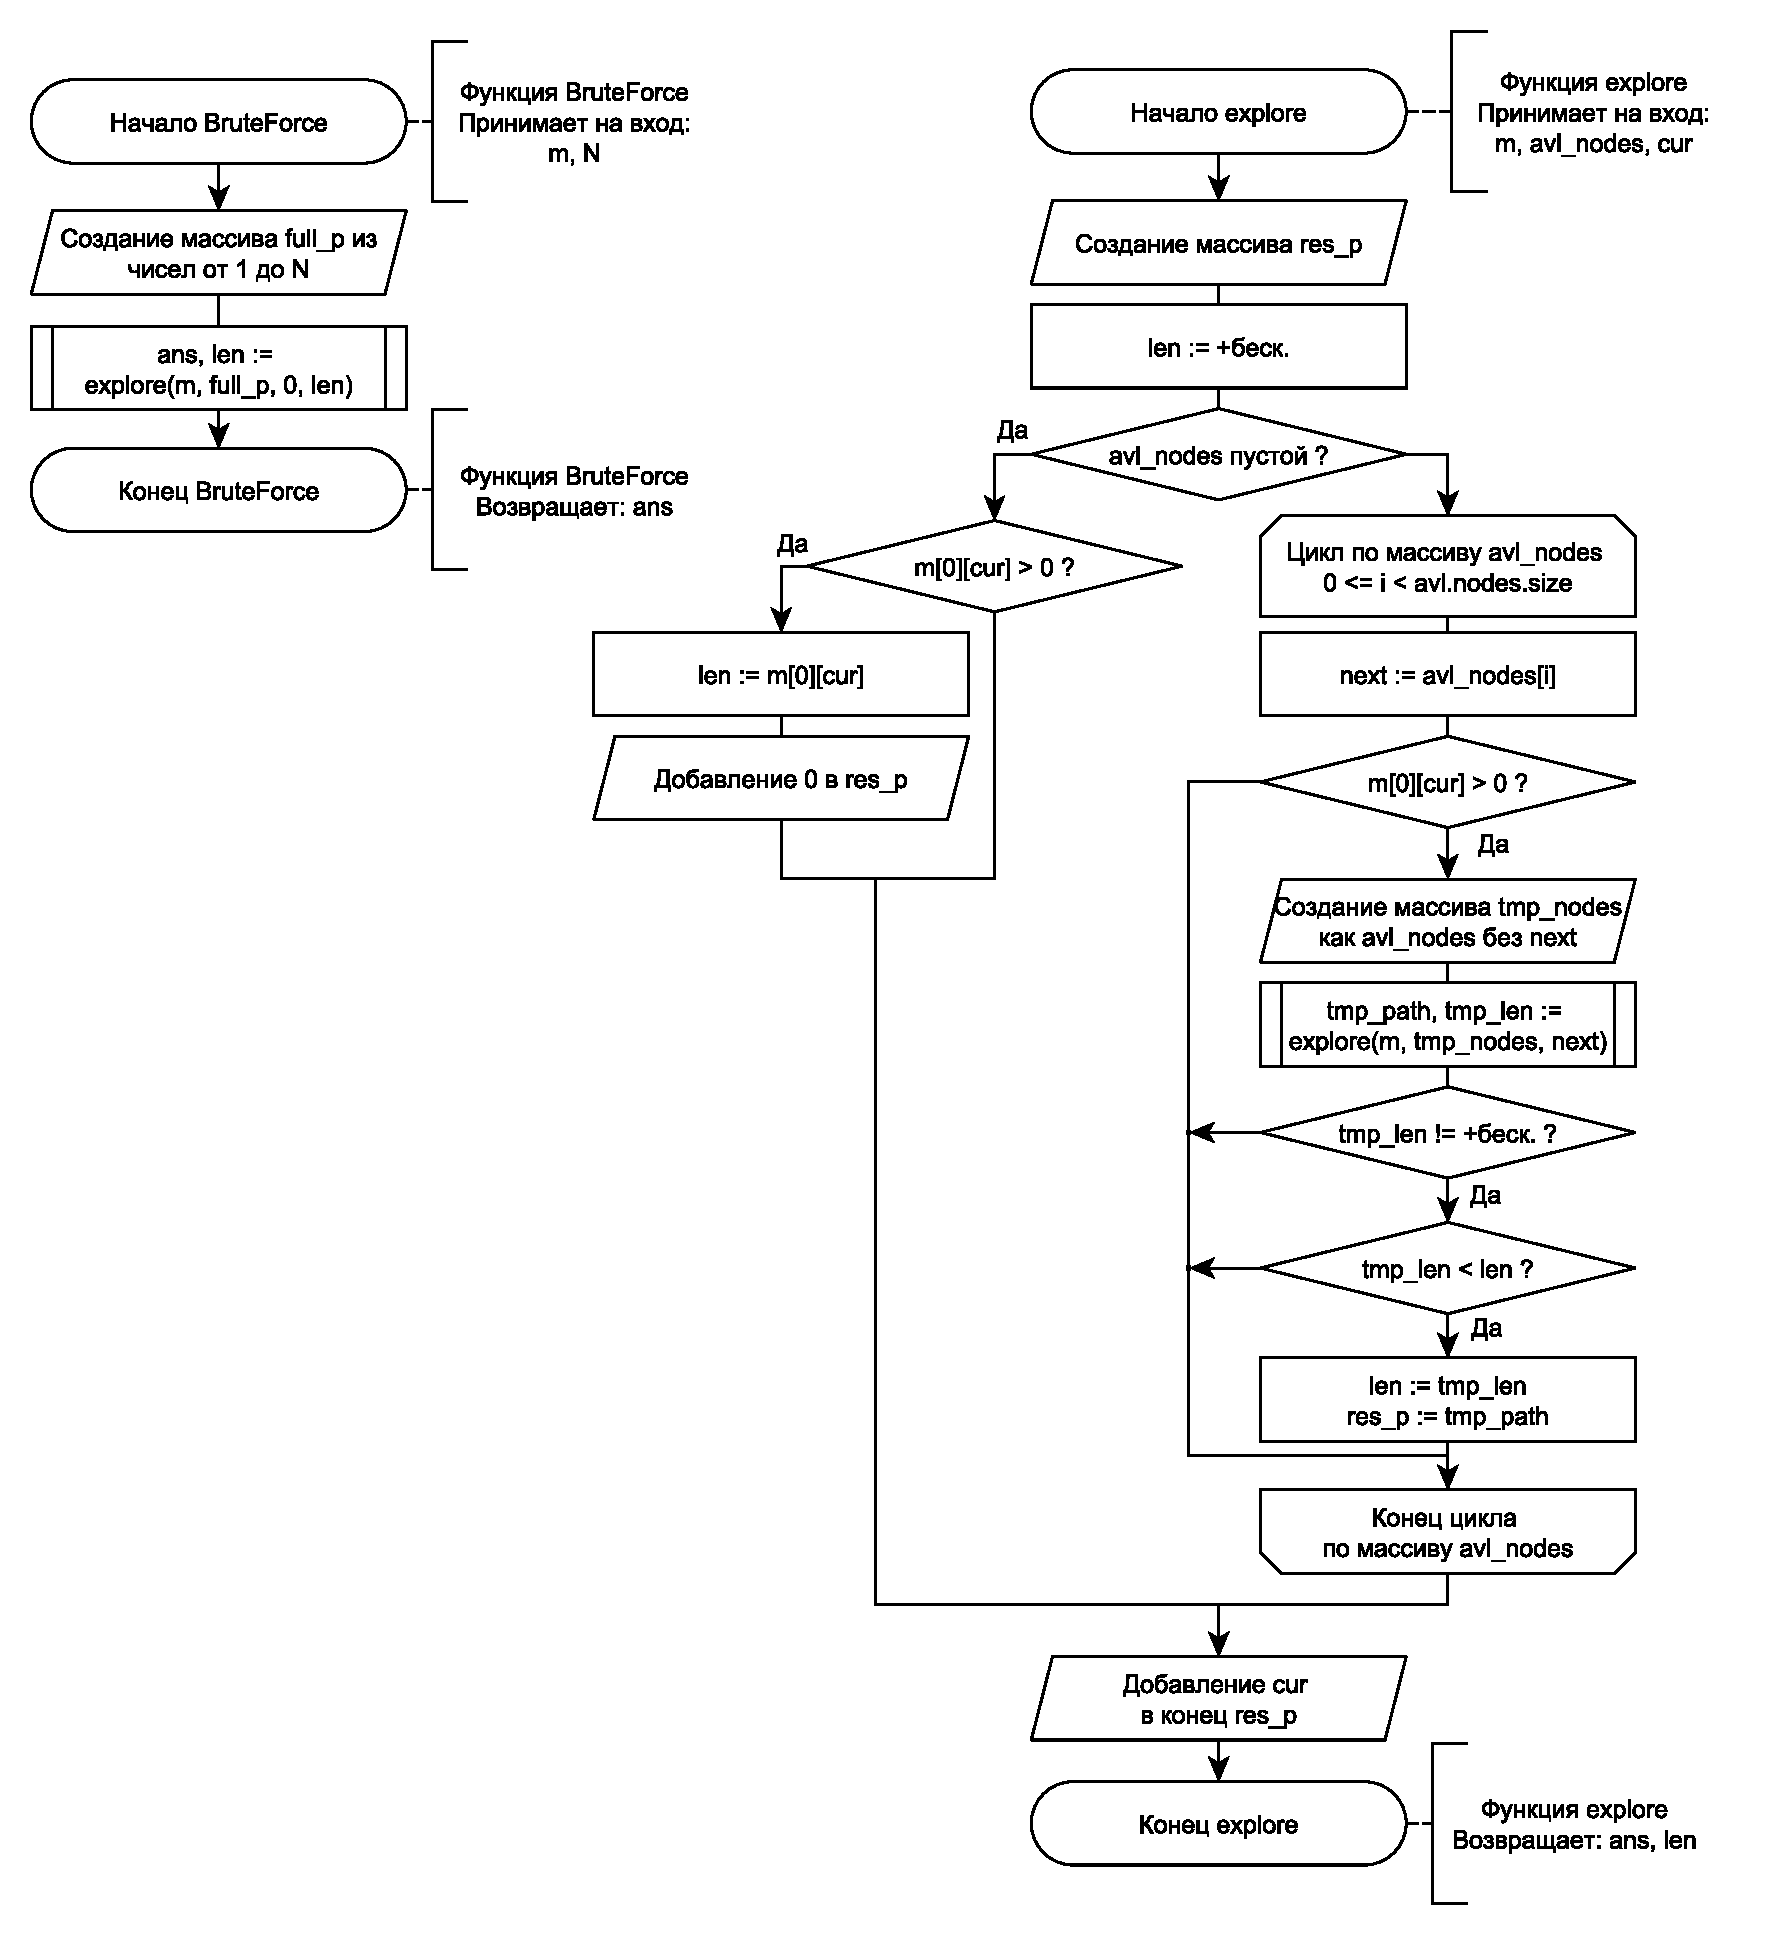
\includegraphics[height=20cm, width = 14cm]{FullSearch}}
		\caption{Поиск полным перебором}
	\end{center}
\end{figure}

\section{Поиск муравьиным алгоритмом}
Изначально создаётся матрица феромонов $tau$, заполненая небольшим положительным числом, минимальный путь и его длина. После этого начинается цикл по дням от 0 до $max_t$.

Каждый муравей содержит информаицю о текущей позиции, проделанном пути и доступных для посещения вершинах. В начале дня создаётся массив муравьёв размером $N$. Каждый из муравьёв помещается в незанятую другим муравьём вершину. Далее производится цикл по каждому из муравьёв.

Для очередного $k$-го муравья осуществляется оценка доступных вершин и переход в одну из них по случайному выбору с найдеными вероятностями. Данные действия повторяются до исчерпания доступных вершин, после чего совершается переход в начальную вершину. В случае, если муравей попадает в тупик, то он останавливается на месте, а результат его прохождения не учитывается далее. В конце пути каждого муравья обновляется значение минимального маршрута.

После конца цикла по муравьям производится создание матрицы $dtau$ приращения феромонов и её заполнение в соответсвии с пройдеными путями. Также симулируется прохождение элитных муравьёв по текущему лучшему пути. После этого производится испарение феромона и занесение значений из $dtau$ в $tau$. Конролируется итоговое значение ячеек $tau$ -- оно не должно опускаться ниже 0.1 от начальной величины.

Схема алгоритма приведена на рисунках 2.2 и 2.3
\begin{figure}[h]
	\begin{center}
		{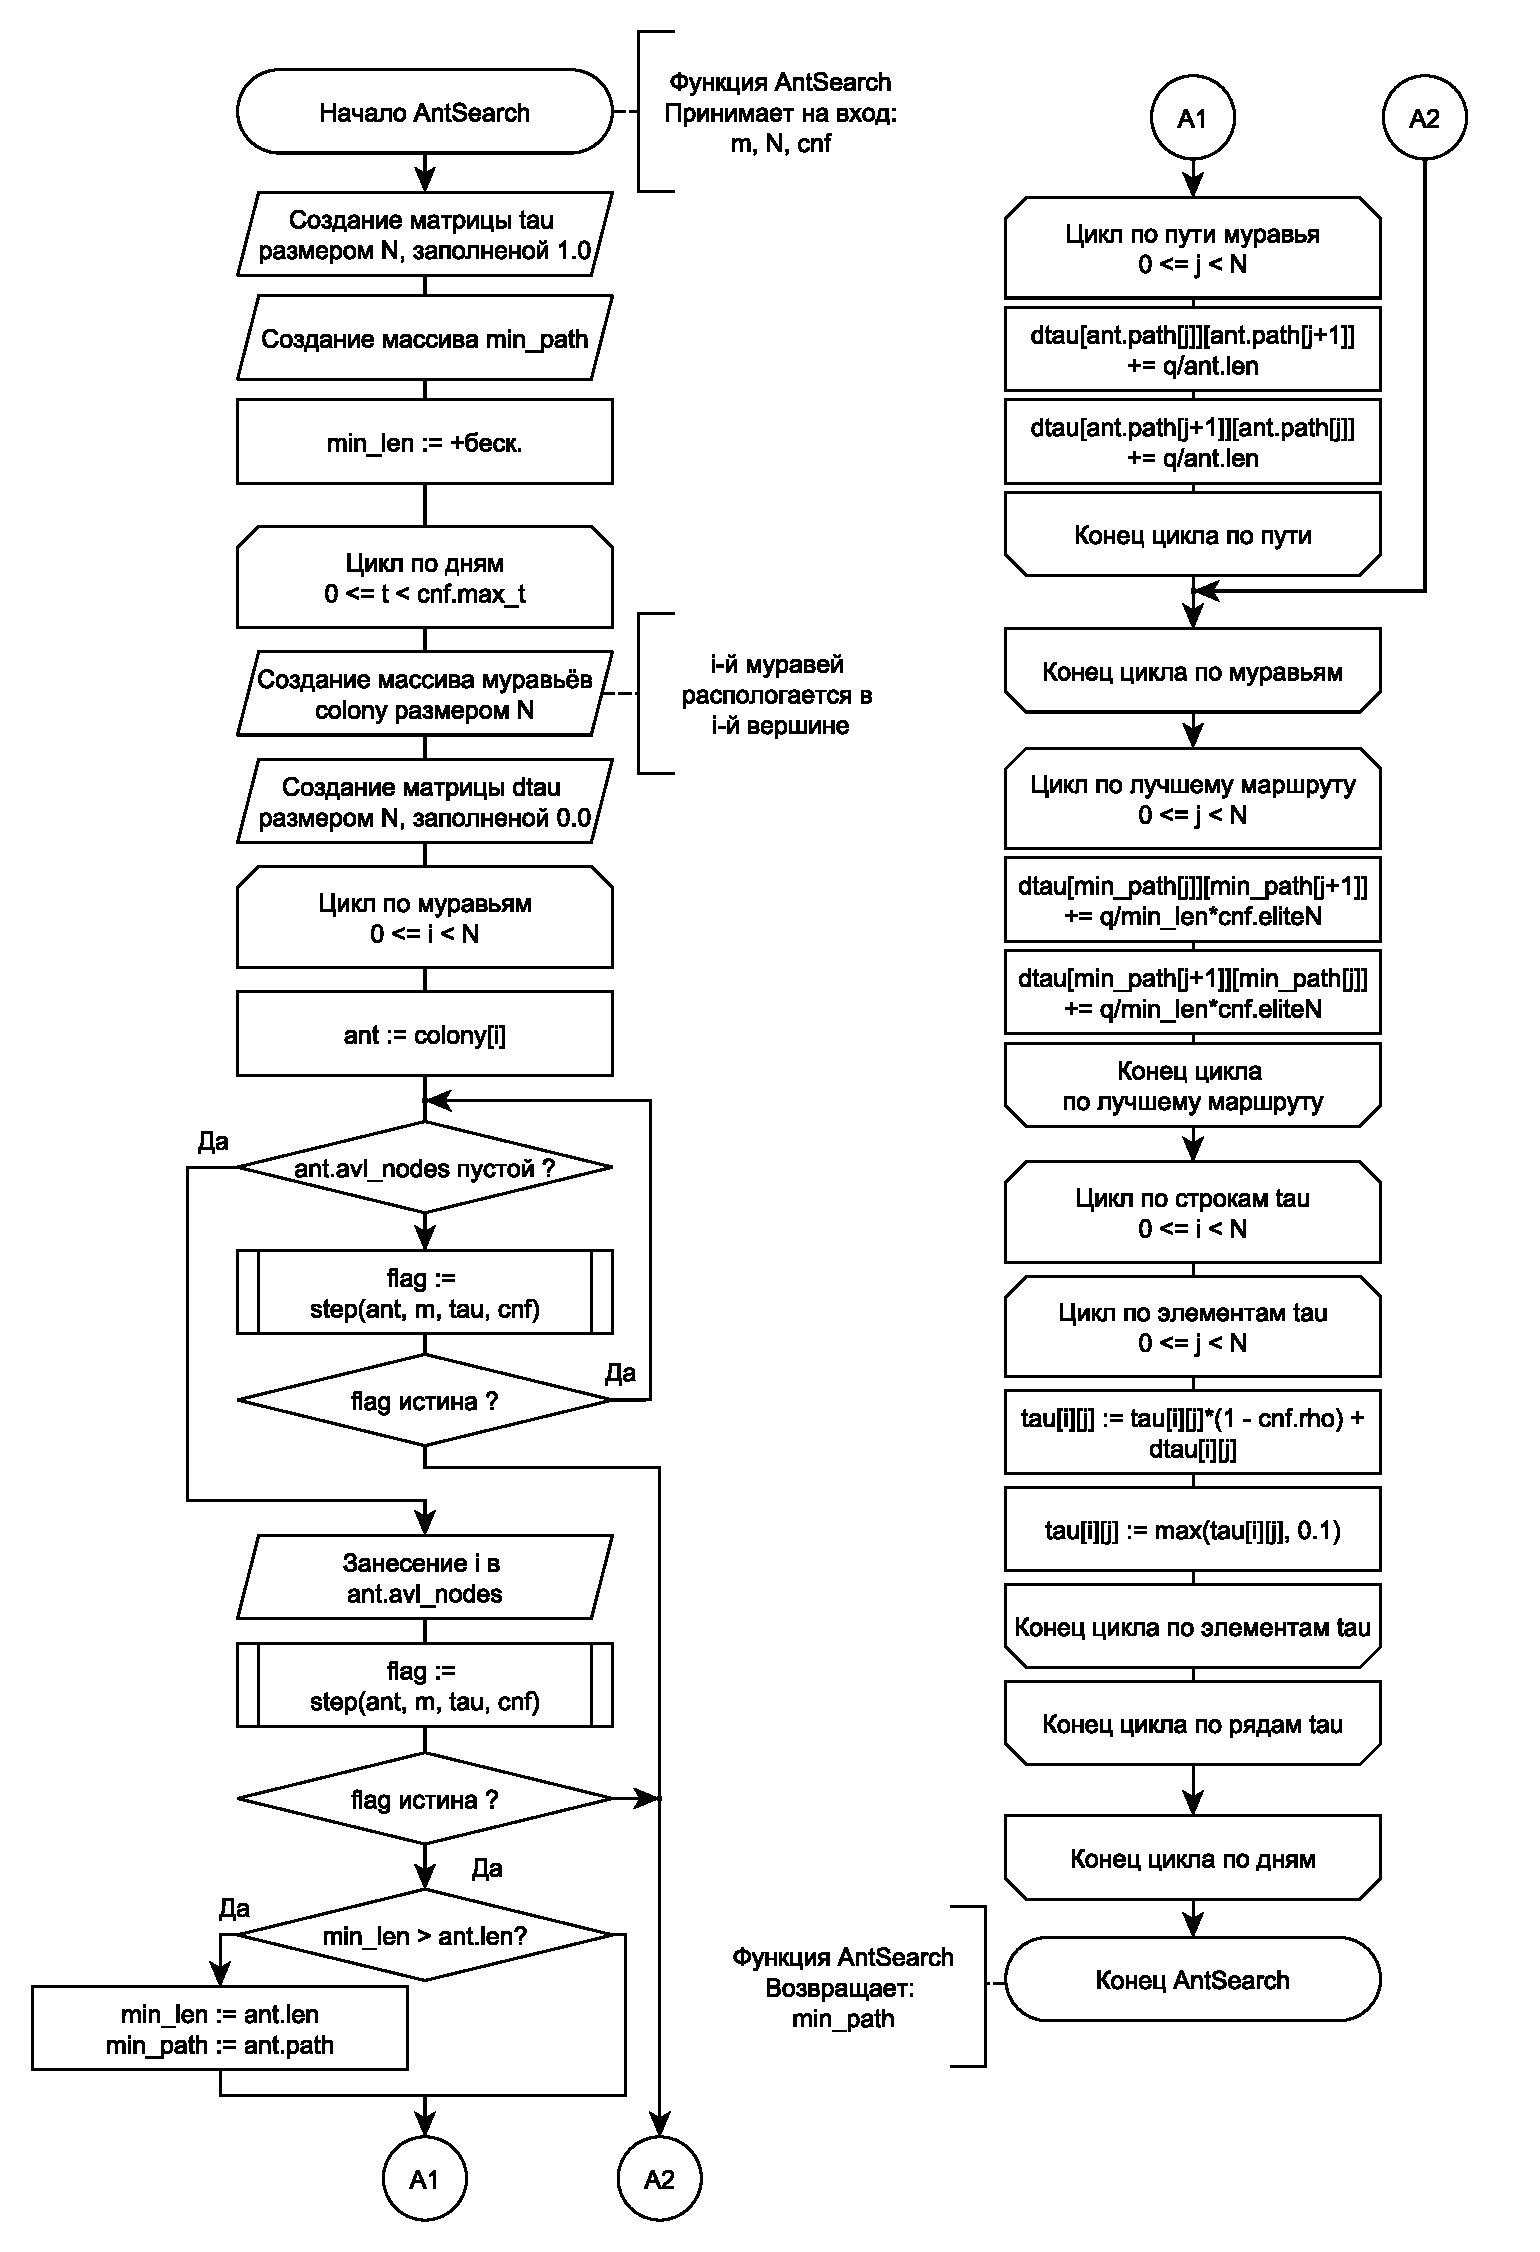
\includegraphics[height=20cm, width = 14cm]{AntMain}}
		\caption{Поиск муравьиным алгоритмом (главная функция)}
	\end{center}
\end{figure}
\begin{figure}[h]
	\begin{center}
		{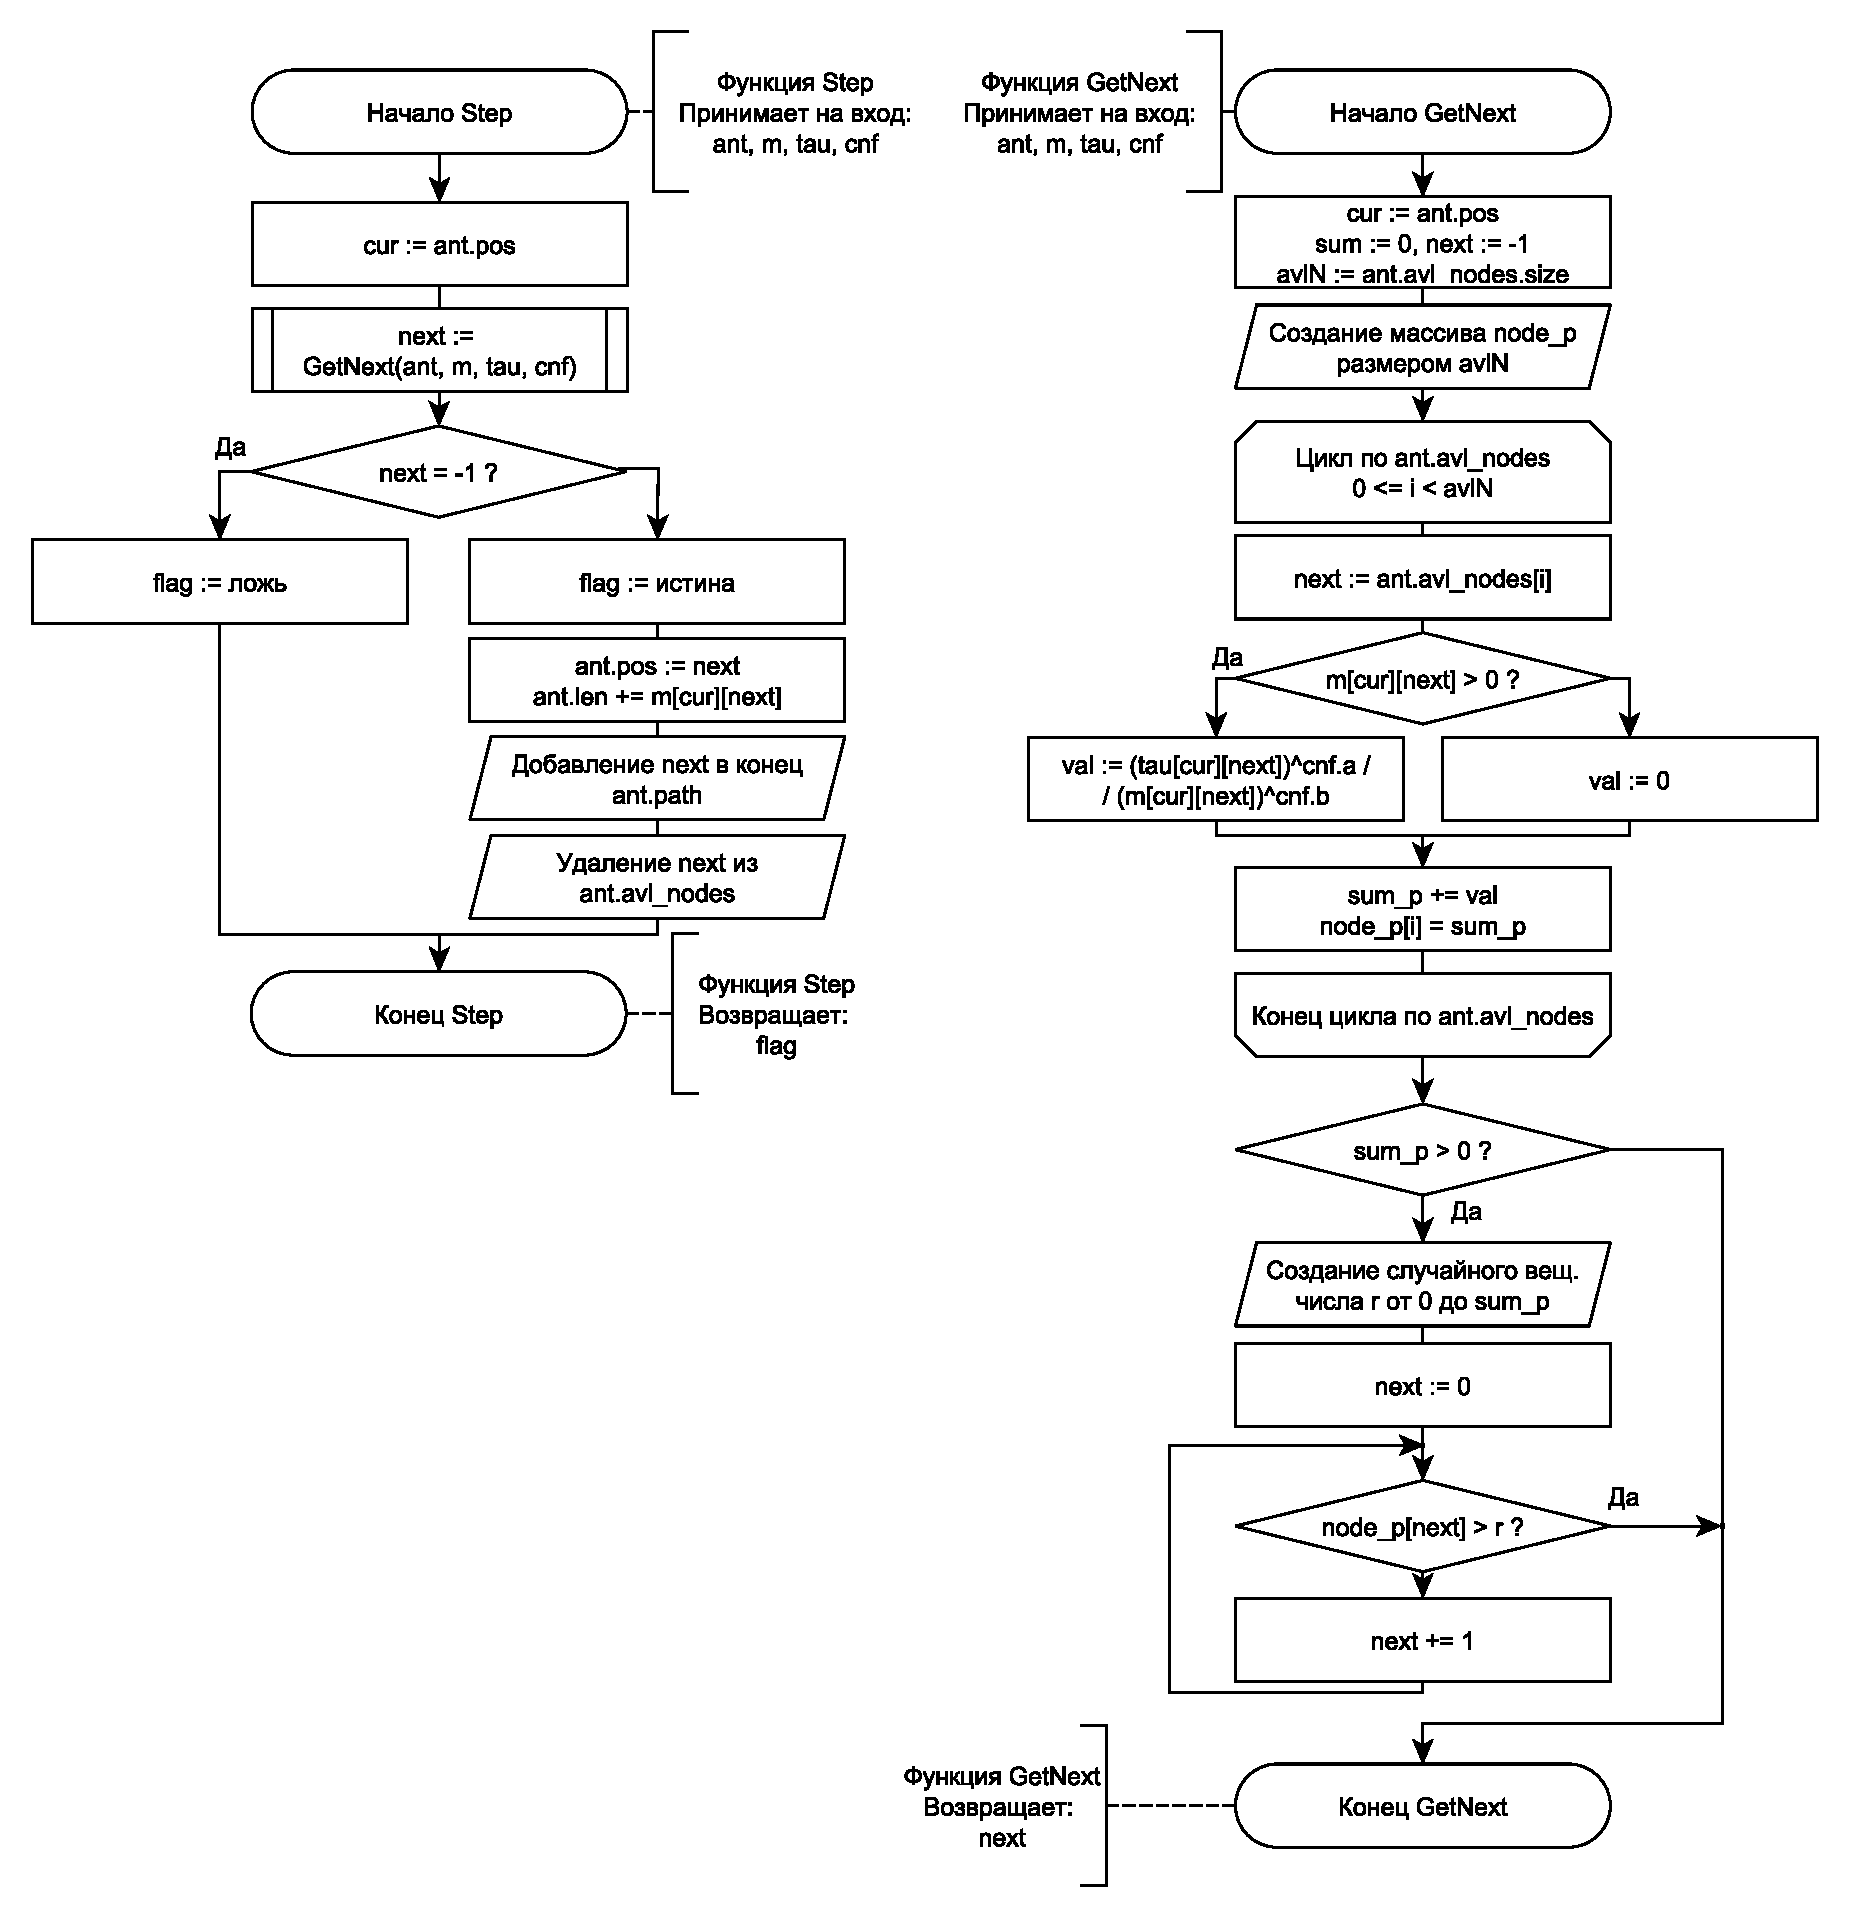
\includegraphics[height=20cm, width = 14cm]{AntStep}}
		\caption{Поиск муравьиным алгоритмом (дополнительные функции)}
	\end{center}
\end{figure}

\section{Автоматическая параметризация муравьиного алгоритма}
Так как муравьиный алгоритм зависит от множества факторов, оптимальные значения используемых параметров могут сильно отличаться в зависимости от класса исследуемого графа. Для поиска наиболее оптимальных параметров требуется создать алгоритм перебора значений параметров, который будет выдавать результат работы для каждого набора и осуществлять поиск наиболее удачных параметров.


\section{Требования к программному обеспечению}
Для полноценной проверки и оценки алгоритмов необходимо выполнить следующее.
\begin{enumerate}
	\item Предоставить возможность ввода матрицы расстояний и проверяемого алгоритма.
	\item Реализовать функцию профилирования, производящую испытания с различными параметрами $\alpha, \beta, \rho$.
\end{enumerate}


\section{Заготовки тестов}
При проверке алгоритма необходимо будет использовать следующие классы тестов:
\begin{itemize}
	\item поиск при двух вершинах;
	\item поиск в графе, где невозможен гамильтонов цикл;
	\item поиск в графе, где все расстояния равны;
	\item поиск в произвольном графе.
\end{itemize}

\section*{Вывод}
Результатом конструторской части стало схематическое описание алгоритмов поиска и параметризации, сформулированны тесты и требования к программному обеспечению.


